\documentclass{article}
%% PACKAGE LOADING

\RequirePackage{geometry}
\RequirePackage[T1]{fontenc}
\RequirePackage{charter}
\RequirePackage{euler}
\RequirePackage{lastpage}
%\RequirePackage[norsk]{babel}
\RequirePackage{enumitem}
\RequirePackage{listings}

\RequirePackage[utf8]{inputenc}     % For utf8 encoded .tex files  % For cross references in pdf
%\RequirePackage[pdftex]{graphicx, hyperref}
\RequirePackage{graphicx}
\RequirePackage{hyperref}
\RequirePackage{color}              % For colouring text  

\hypersetup{colorlinks=true,     
		linkcolor=blue,          % color of internal links (change box color with linkbordercolor)
    citecolor=blue,        % color of links to bibliography
    filecolor=blue,      % color of file links
    urlcolor=blue           % color of external links
		}
\setlist[enumerate]{itemsep=0mm, topsep=5pt, partopsep=0mm, parsep=0mm}
\setlist[enumerate,1]{label=\arabic*., ref=\arabic*}
\setlist[enumerate,2]{label=\arabic*., ref=\arabic*}
\setlist[enumerate,3]{label=\alph*., ref=\alph*}
\setlist[itemize]{itemsep=0mm, topsep=5pt, partopsep=0mm, parsep=0mm}
\setlist[itemize,1]{label=$\bullet$}
\setlist[itemize,2]{label=$\circ$}
\setlist[itemize,3]{label=$\cdot$}
%\RequirePackage[absolute]{textpos}

\usepackage{csvsimple}
\usepackage{booktabs}

\usepackage{gnuplottex}


\definecolor{darkgreen}{rgb}{0,0.5,0}
\definecolor{darkred}{rgb}{0.5,0.0,0}

\lstset{        basicstyle=\ttfamily,
                keywordstyle=\color{blue}\ttfamily,
                stringstyle=\color{darkred}\ttfamily,
                commentstyle=\color{darkgreen}\ttfamily,
}


%Typesetting of C++
\newcommand{\CPP}[0]{{C\nolinebreak[4]\hspace{-.1em}\raisebox{.1ex}{\small\bf +\hspace{-.1em}+\ }}}



%\newcommand{\comment}[1]{\textcolor{blue}{\emph{#1}}}  %% use of the colour and you can see how to use commands with parts \comment{so what}

%% The class files defines these two
%% \newcommand{\NTNU}{Norwegian University for Science and Technology} %

% you can create you one #define like structures using the \newcommand feature
% you can change behaviour using \renewcommand

\newcommand{\com}[1]{{\color{red}#1}} % supervisor comment
%\renewcommand{\com}[1]{} %remove starting % to remove supervisor comments
% This will appear in text \com{Lectures comment} and be visible unless you uncomment
% the renewcommand line.

\newcommand{\todo}[1]{{\color{green}#1}} % items to do
%\renewcommand{\todo}[1]{} %remove starting % to remove items to do

\newcommand{\n}[1]{{\color{blue}#1}} % other comment
%\renewcommand{\n}[1]{} %remove starting % to remove notes

\newcommand{\dn}[1]{} % add the d to a note to say that you have finished with it.

\newcommand{\gj}{NTNU i Gj\o{}vik}



\title{IMT3601 Game Programming - \\ \todo{Your title here}}
\author{Simon McCallum, Marius Nowostawski}
\date{December 2017}


\usepackage{natbib}
\usepackage{graphicx}

\begin{document}

\maketitle


\section{Pitch}
\label{sec:pitch}
This is the short description of the game you developed.  Think of it at what might appear on Steam or on the back of the box of the game.  This could be similar to the pitch you gave the first year students. You could include multiple screen shots.

\begin{figure}[h!]
\centering
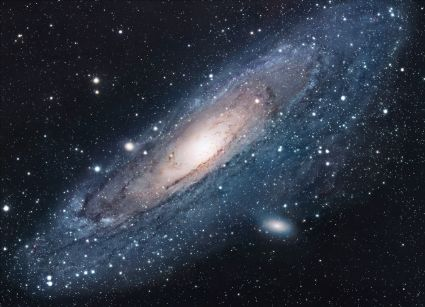
\includegraphics[scale=1.7]{images/universe.jpg}
\caption{Screenshot from Level X }
\label{fig:univerise}
\end{figure}


\section{Team}
\label{sec:team}

\begin{tabular}{lll}
Student         & Role          & Area of Responsibility \\ \hline
Simon McCallum  & Design Lead   & Course overveiw\\
Mariusz Nowostawski & Tech Lead & Netorking \\
Christopher Frantz & Intern     & Population Simulation\\
\end{tabular}

\section{Links}

\todo{In this section you should include the links to the repositories with code and also any executable or videos we should watch}



\section{Implementation}
\label{sec:implementation}

This section describes what you have implemented focusing on what is the most challenging aspects of the development.

\subsection{Development Environment}

What environment you used which might be connected to the section below on technology if the two are linked

\subsection{Technology}

The technology you used to develop the game, the engine or libraries


\subsection{External Dependencies}
Other tools that your game relies on

\subsection{Architecture}
A brief overview of the architecture of the game you made





The subsections should include content on the interesting decisions you had to make and why you made them.  This is an opportunity for you to reflect on the project and what you learnt and why you did what you ended up doing.


\subsection{}

\section{Conclusion}
``I always thought something was fundamentally wrong with the universe'' \citep{adams1995hitchhiker}

\bibliographystyle{plain}
\bibliography{references}
\end{document}
